        %%******************************************%%
        %%                                          %%
        %%        Modello di tesi di laurea         %%
        %%            di Andrea Giraldin            %%
        %%                                          %%
        %%             2 novembre 2012              %%
        %%                                          %%
        %%******************************************%%

\begin{document}
    \frontmatter
    \begin{titlepage}
    \begin{center}
        \begin{LARGE}
            \textbf{\myUni}\\
        \end{LARGE}

        \vspace{10pt}

        \begin{Large}
            \textsc{\myDepartment}\\
        \end{Large}

        \vspace{10pt}

        \begin{large}
            \textsc{\myFaculty}\\
        \end{large}

        \vspace{30pt}
        \begin{figure}[htbp]
            \centering
            
\includegraphics[height=6cm]{unipd-logo}
        \end{figure}
        \vspace{30pt}

        \begin{LARGE}
            \textbf{\myTitle}\\
        \end{LARGE}

        \vspace{10pt}

        \begin{large}
            \textsl{\myDegree}\\
        \end{large}

        \vspace{40pt}

        \begin{large}
            \begin{flushleft}
                \textit{Relatore}\\
                \vspace{5pt}
                Prof.ssa \myProf
            \end{flushleft}

            % You can tweak the spacing to have professor and student names on the same line
            % useful if the page is broken by a long thesis title and you need more space
            % \vspace{-52pt}

            \begin{flushright}
                \textit{Laureando}\\
                \vspace{5pt}
                \myName \\
                2009116
            \end{flushright}
        \end{large}

        \vspace{30pt}

        \line(1, 0){338} \\
        \begin{normalsize}
            \textsc{Anno Accademico \myAA}
        \end{normalsize}
    \end{center}
\end{titlepage}

    \clearpage
\phantomsection
\thispagestyle{empty}

\hfill
\vfill

\noindent\myName: \textit{\myTitle,}
\myDegree,
\textcopyright\ \myTime.

    \cleardoublepage
\phantomsection
\thispagestyle{empty}
\pdfbookmark{Dedica}{Dedica}

\vspace*{3cm}

\begin{center}
    Lorem ipsum dolor sit amet, consectetuer adipiscing elit. \\ \medskip
    --- Oscar Wilde
\end{center}

\medskip

\begin{center}
    Dedicato a ...
\end{center}

    \cleardoublepage
\phantomsection
\pdfbookmark{Sommario}{Sommario}
\begingroup
\let\clearpage\relax
\let\cleardoublepage\relax
\let\cleardoublepage\relax

\chapter*{Sommario}
Il presente documento descrive il lavoro svolto durante il periodo di stage, della durata di circa trecentoventi ore, dal laureando Michael Amista' presso l'azienda CWBI (Codice Web Banking Innovation).

\setlength{\parskip}{3ex}

\noindent L'obiettivo dello stage riguarda lo sviluppo di un modulo web per una webapp aziendale preesistente. In particolare ciò che è stato sviluppato è un sistema di gestione delle campagne a supporto dell'area marketing in un contesto bancario/fintech. Vincolo di sviluppo sono le metodologie di analisi, progettazione e sviluppo aziendale, oltre allo stack tecnologico utilizzato dall'azienda. Viene inoltre riportata un'analisi finale che pone a confronto le aspettative iniziali personali con quelli che sono stati i risultati finali e gli obiettivi raggiunti.

\endgroup

\vfill

    \cleardoublepage
\phantomsection
\pdfbookmark{Ringraziamenti}{ringraziamenti}

\begin{flushright}{
    \slshape
    ``Life is really simple, but we insist on making it complicated''} \\
    \medskip
    --- Confucius
\end{flushright}


\bigskip

\begingroup
\let\clearpage\relax
\let\cleardoublepage\relax
\let\cleardoublepage\relax

\chapter*{Ringraziamenti}

\noindent \textit{Innanzitutto, vorrei esprimere la mia gratitudine al Prof. \myProf, relatore della mia tesi, per l'aiuto e il sostegno fornitomi durante la stesura del lavoro.}\\

\noindent \textit{Desidero ringraziare con affetto i miei genitori per il sostegno, il grande aiuto e per essermi stati vicini in ogni momento durante gli anni di studio.}\\

\noindent \textit{Ho desiderio di ringraziare poi i miei amici per tutti i bellissimi anni passati insieme e le mille avventure vissute.}\\
\bigskip

\noindent\textit{\myLocation, \myTime}
\hfill \myName

\endgroup

    \cleardoublepage
\pdfbookmark{\contentsname}{tableofcontents}
\setcounter{tocdepth}{2}
\tableofcontents
%\markboth{\contentsname}{\contentsname}
\clearpage

\begingroup
    \let\clearpage\relax
    \let\cleardoublepage\relax
    \let\cleardoublepage\relax

    % Figures list
    \phantomsection
    \pdfbookmark{\listfigurename}{lof}
    \listoffigures

    \vspace*{8ex}

    % Tables list
    \phantomsection
    \pdfbookmark{\listtablename}{lot}
    \listoftables

    \vspace*{8ex}
\endgroup

\cleardoublepage

    \cleardoublepage

    \mainmatter
    \chapter{Introduzione}
\label{cap:introduzione}

\intro{Il seguente capitolo ha la funzione di introdurre l'azienda ospitante presso la quale è stato svolto lo stage. Vengono inoltre elencate quelle che sono le aspettative personali principalmente riguardo la crescita tecnica e professionale.}

\setlength{\parskip}{3ex}

\section{L'azienda}

\begin{figure}[!h]
	\centering
	
\includegraphics[width=6cm]{../images/CWBI-logo.png}
	\caption{Logo azienda CWBI}
\end{figure}

\setlength{\parskip}{3ex}

\noindent CWBI (Codice Web Banking Innovation) è un’azienda italiana che opera nel mercato dell'Information Communication Technology e supporta i propri clienti nello studio dei modelli di business, nella definizione dei processi organizzativi e nella progettazione e realizzazione di software con un forte orientamento alle nuove tecnologie.

\setlength{\parskip}{3ex}

\noindent Fondata a Padova nell'anno 2013, CWBI ha fidelizzato rapporti di collaborazione con aziende nazionali di primaria importanza attraverso la sua struttura interna costituita da professionisti con skills elevate, che negli anni hanno maturato un forte know-how in diversi settori di business quali: Banking, Media and Publishing, Insurance, Industry.

\setlength{\parskip}{3ex}

\noindent Anni di esperienza permettono all'azienda di affrontare con successo ogni singolo aspetto del ciclo di vita dei progetti nei quali è coinvolta; entusiasmo e visione strategica, accompagnati da un forte orientamento al risultato, sono il motore della sua capacità innovativa.

\setlength{\parskip}{3ex}

\noindent CWBI offre una vasta gamma di servizi, tra cui:
\begin{itemize}
\item sviluppo di applicazioni e portali web-based;
\item sviluppo di applicazioni mobile;
\item studio di fattibilità e sostenibilità dei modelli di business;
\item analisi e definizione dei processi organizzativi;
\item studi di navigabilità e usabilità;
\item studi di ergonomia del software.
\end{itemize}

\section{Aspettative personali}
L'obiettivo dell'attività di stage, oltre lo sviluppo del progetto commissionato dall'azienda ospitante, è quello di crescere personalmente e professionalmente tramite un'impronta aziendale caratterizzata da competenza tecnica e professionale.

\setlength{\parskip}{3ex}

\noindent Di seguito vengono riportati gli obiettivi personali a titolo professionale e formativo da raggiungere:
\begin{itemize}
\item apprendimento di Java;
\item apprendimento dei framework Spring e Hibernate;
\item apprendimento di HTML5/CSS3 e del framework Bootstrap;
\item apprendimento JavaScript e della libreria jQuery;
\item apprendimento del sistema di controllo di versione aziendale;
\item apprendimento dei processi aziendali;
\item apprendimento degli strumenti per la gestione di progetto;
\item apprendimento dell’ambiente di sviluppo;
\item studio di fattibilità del progetto e realizzazione dello stesso le tecnlogie aziendali;
\item capacità di trovare soluzioni alternative da quelle proposte.
\end{itemize}

\section{Organizzazione del testo}


{\hyperref[cap:descrizione-stage]{Il secondo capitolo}} descrive l'attività di stage definendo il problema da affrontare e i vincoli da rispettare lungo lo sviluppo.
    
\noindent {\hyperref[cap:analisi-requisiti]{Il terzo capitolo}} approfondisce l'analisi dei requisiti effettuata, elencando i casi d'uso raccolti e definendo i rispettivi requisiti.
    
\noindent {\hyperref[cap:strumenti-utilizzati]{Il quarto capitolo}} approfondisce gli strumenti e le tecnologie utilizzate nello sviluppo del prodotto commissionato e che si pongono come vincolo di progetto.
    
\noindent {\hyperref[cap:progettazione]{Il quinto capitolo}} approfondisce la progettazione, caratterizzata dall'architettura del sistema e dai design pattern utilizzati.
    
\noindent {\hyperref[cap:prodotto-finale]{Il sesto capitolo}} illustra il prodotto finale in tutte le sue componenti.
    
\noindent {\hyperref[cap:conclusioni]{Nel settimo capitolo}} si possono trovare le conclusioni sul lavoro svolto e formate dai test effettuati e da un resoconto finale che pone a confronto le aspettative iniziali con quelli che sono stati i traguardi raggiunti al termine dell'esperienza di stage.

\noindent Riguardo la stesura del testo, relativamente al documento sono state adottate le seguenti convenzioni tipografiche:
\begin{itemize}
	\item gli acronimi, le abbreviazioni e i termini ambigui o di uso non comune menzionati vengono definiti nel glossario, situato alla fine del presente documento;
	\item per la prima occorrenza dei termini riportati nel glossario viene utilizzata la seguente nomenclatura: \emph{parola}\glsfirstoccur.
\end{itemize}

    \chapter{Processi e metodologie}
\label{cap:processi-metodologie}

\intro{Brevissima introduzione al capitolo}\\

\section{Processo sviluppo prodotto}

    \chapter{Descrizione dello stage}
\label{cap:descrizione-stage}

\intro{Breve introduzione al capitolo}\\

\section{Introduzione al progetto}

\section{Analisi preventiva dei rischi}

Durante la fase di analisi iniziale sono stati individuati alcuni possibili rischi a cui si potrà andare incontro.
Si è quindi proceduto a elaborare delle possibili soluzioni per far fronte a tali rischi.\\

\begin{risk}{Performance del simulatore hardware}
    \riskdescription{le performance del simulatore hardware e la comunicazione con questo potrebbero risultare lenti o non abbastanza buoni da causare il fallimento dei test}
    \risksolution{coinvolgimento del responsabile a capo del progetto relativo il simulatore hardware}
    \label{risk:hardware-simulator} 
\end{risk}

\section{Requisiti e obiettivi}


\section{Pianificazione}

    \chapter{Analisi dei requisiti}
\label{cap:analisi-requisiti}

\intro{Breve introduzione al capitolo}\\

\section{Casi d'uso}

Per lo studio dei casi di utilizzo del prodotto sono stati creati dei diagrammi.
I diagrammi dei casi d'uso (in inglese \emph{Use Case Diagram}) sono diagrammi di tipo \gls{uml} dedicati alla descrizione delle funzioni o servizi offerti da un sistema, così come sono percepiti e utilizzati dagli attori che interagiscono col sistema stesso.
Essendo il progetto finalizzato alla creazione di un tool per l'automazione di un processo, le interazioni da parte dell'utilizzatore devono essere ovviamente ridotte allo stretto necessario. Per questo motivo i diagrammi d'uso risultano semplici e in numero ridotto.

\begin{figure}[!h] 
    \centering 
    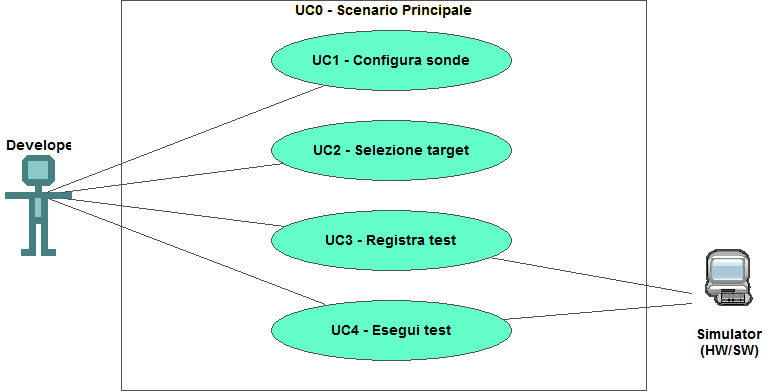
\includegraphics[width=0.9\columnwidth]{usecase/scenario-principale} 
    \caption{Use Case - UC0: Scenario principale}
\end{figure}

\begin{usecase}{0}{Scenario principale}
\usecaseactors{Sviluppatore applicativi}
\usecasepre{Lo sviluppatore è entrato nel plug-in di simulazione all'interno dell'IDE}
\usecasedesc{La finestra di simulazione mette a disposizione i comandi per configurare, registrare o eseguire un test}
\usecasepost{Il sistema è pronto per permettere una nuova interazione}
\label{uc:scenario-principale}
\end{usecase}

\section{Tracciamento dei requisiti}

Da un'attenta analisi dei requisiti e degli use case effettuata sul progetto è stata stilata la tabella che traccia i requisiti in rapporto agli use case.\\
Sono stati individuati diversi tipi di requisiti e si è quindi fatto utilizzo di un codice identificativo per distinguerli.\\
Il codice dei requisiti è così strutturato R(F/Q/V)(N/D/O) dove:
\begin{enumerate}
	\item[R =] requisito
    \item[F =] funzionale
    \item[Q =] qualitativo
    \item[V =] di vincolo
    \item[N =] obbligatorio (necessario)
    \item[D =] desiderabile
    \item[Z =] opzionale
\end{enumerate}
Nelle tabelle \ref{tab:requisiti-funzionali}, \ref{tab:requisiti-qualitativi} e \ref{tab:requisiti-vincolo} sono riassunti i requisiti e il loro tracciamento con gli use case delineati in fase di analisi.

\newpage

\begin{table}%
\caption{Tabella del tracciamento dei requisti funzionali}
\label{tab:requisiti-funzionali}
\begin{tabularx}{\textwidth}{lXl}
\hline\hline
\textbf{Requisito} & \textbf{Descrizione} & \textbf{Use Case}\\
\hline
RFN-1     & L'interfaccia permette di configurare il tipo di sonde del test & UC1 \\
\hline
\end{tabularx}
\end{table}%

\begin{table}%
\caption{Tabella del tracciamento dei requisiti qualitativi}
\label{tab:requisiti-qualitativi}
\begin{tabularx}{\textwidth}{lXl}
\hline\hline
\textbf{Requisito} & \textbf{Descrizione} & \textbf{Use Case}\\
\hline
RQD-1    & Le prestazioni del simulatore hardware deve garantire la giusta esecuzione dei test e non la generazione di falsi negativi & - \\
\hline
\end{tabularx}
\end{table}%

\begin{table}%
\caption{Tabella del tracciamento dei requisiti di vincolo}
\label{tab:requisiti-vincolo}
\begin{tabularx}{\textwidth}{lXl}
\hline\hline
\textbf{Requisito} & \textbf{Descrizione} & \textbf{Use Case}\\
\hline
RVO-1    & La libreria per l'esecuzione dei test automatici deve essere riutilizzabile & - \\
\hline
\end{tabularx}
\end{table}%

    \chapter{Progettazione e codifica}
\label{cap:progettazione-codifica}

\intro{Breve introduzione al capitolo}\\

\section{Tecnologie e strumenti}
\label{sec:tecnologie-strumenti}

Di seguito viene data una panoramica delle tecnologie e strumenti utilizzati.

\subsection*{Tecnologia 1}
Descrizione Tecnologia 1.

\subsection*{Tecnologia 2}
Descrizione Tecnologia 2

\section{Ciclo di vita del software}
\label{sec:ciclo-vita-software}

\section{Progettazione}
\label{sec:progettazione}

\subsubsection{Namespace 1} %**************************
Descrizione namespace 1.

\begin{namespacedesc}
    \classdesc{Classe 1}{Descrizione classe 1}
    \classdesc{Classe 2}{Descrizione classe 2}
\end{namespacedesc}


\section{Design Pattern utilizzati}

\section{Codifica}

    \chapter{Verifica e validazione}
\label{cap:verifica-validazione}

    \chapter{Conclusioni}
\label{cap:conclusioni}

\section{Consuntivo finale}

\section{Raggiungimento degli obiettivi}

\section{Conoscenze acquisite}

\section{Valutazione personale}


    \appendix
    \chapter{Appendice A}

\epigraph{Citazione}{Autore della citazione}


    \backmatter
    \printglossary[type=\acronymtype, title=Acronimi e abbreviazioni, toctitle=Acronimi e abbreviazioni]
    \printglossary[type=main, title=Glossario, toctitle=Glossario]

    \cleardoublepage
\chapter{Sitografia}
\label{cap:sitografia}
\nocite{*}

% Print book bibliography
\printbibliography[heading=subbibliography,title={Riferimenti bibliografici},type=book]

% Print site bibliography
\printbibliography[heading=subbibliography,title={Siti web consultati},type=online]

\paragraph*{Spring} \url{https://spring.io/}
\label{para:spring-site}

\paragraph*{Hibernate} \url{https://hibernate.org/}
\label{para:hibernate-site}

\paragraph*{Bootstrap} \url{https://getbootstrap.com/}
\label{para:bootstrap-site}

\paragraph*{Apache Struts} \url{https://struts.apache.org/}
\label{para:struts-site}

\paragraph*{Apache Commons} \url{https://commons.apache.org/}
\label{para:commons-site}
\end{document}
